\section{Methods}

\subsection{General consideration and assumptions}\label{sec:generalconsiderations}

\subsubsection{Collagen fibrils and fibers} \label{sec:collagenconsiderations}

    In the present work, we assumed that the collagen fibrils were contiguous subunits of the collagen fibers so that there was negligible slippage between fibrils. To characterize the straightening behavior of the fiber-level crimped structure \cite{lanir_constitutive_1983, fata_insights_2014, sacks_incorporation_2003, lanir_structural_1979, kastelic_structural_1980, hansen_recruitment_2002, cacho_constitutive_2007, grytz_constitutive_2009}, we use only the fiber axial stretch needed to fully straighten the fiber, slack stretch, rather than the period and amplitude of the collagen fibers. This avoids the necessity of incorporating detailed unloaded geometry for the collagen fibers.


    In most structural models, the distribution of collagen slack strains (the recruitment distribution) is assumed to be independent of the orientation. This approach has the advantage of allowing collagen fiber recruitment model parameters to be determined directly from a single planar equibiaxial strain (EB) tests, where the deformation gradient tensor is $F = \operatorname{diag}[\lambda, \lambda, 1/\lambda^2$] and no fiber rotations occur (e.g. \cite{fata_insights_2014}). For bovine pericardium, we have shown that when the collagen fiber orientation distribution function (ODF) is obtained independently, the complete in-plane response can be predicted \cite{sacks_incorporation_2003}. However, some angular dependence may be physiologically relevant for general tissues. For example, collagen fibers are constantly produced and degraded under physiological stresses and prefer to function within homeostatic stress levels \cite{humphrey_cardiovascular_2002}. Moreover, MV leaflets experience large and highly anisotropic deformations in vivo, which would induce substantially higher fiber ensemble stresses in the larger strain direction \cite{amini_vivo_2012,sacks_vivo_2006}. We thus speculate that collagen fibers may exhibit larger undulations in the directions of larger physiological strain to maintain a constant fiber ensemble stress. However, the exact dependence of collagen recruitment on fiber orientation remains unknown and has yet to be explored in the literature.

    
    For the collagen fiber material model, a stress-strain relation that is linear in 2nd Piola Kirchhoff stress and Green Lagrange strain is the predominant fiber model of choice \cite{sacks_incorporation_2003,lanir_structural_1979,fan_simulation_2014}. However, SAXS studies of intact tissue shows that the fibril strain varies linearly with applied forces in tendon \cite{sasaki_elongation_1996,sasaki_stress_1996} and MV leaflet tissues \cite{liao_relation_2007}. Furthermore, the results are corroborated by the atomistic modeling results by Buehler \cite{buehler_atomistic_2006}, where the force-displacement relation is essentially linear at strains lower than 0.35.
    



\subsubsection{Elastin fiber network} \label{sec:elastinconsiderations}

    Elastin fibers function through an entropy-driven process wherein the decrease in entropy drives the increase in fiber stress as the fiber is elongated. As of yet, there is no first-principle form for elastin when modeled either as a continuous phase or a discrete fibrous network. Typical MV models are either purely phenomenological or ignore the elastin component entirely. In a previous study on ovine pulmonary artery \cite{fata_insights_2014}, we found the elastin fibers to behave linearly in second Piola–Kirchhoff stress and Green Lagrange strain. However, the specific form of the elastin likely depends on a variety of factors including cross-linking and residual strain. Moreover, it is not clear if there are layer-specific differences, and thus a more general material model for the MV elastin fiber network is needed.




\subsubsection{Affine kinematics and layer averaged responses}

    As in previous structural approaches, we assume affine fiber kinematics. This assumption is supported by a recent study wherein we demonstrated that the MV anterior leaflet collagen and elastin fibers all deformed in a manner consistent with affine deformation kinematics \cite{lee_presence_2015}. We further assume each layer is structurally homogeneous (i.e. ignore intra-layer structural variations). Thus, and in order to derive the total individual layer response as a function of its collagen and elastin components, the following information was used (Table \ref{c2tab:experiments}):
        \begin{enumerate}
            \item The mass composition of each layer, including the quantities of collagen and elastin.
            \item The ODF for the collagen and elastin fibers within each layer.
            \item The recruitment behaviors of the collagen fiber network for each layer.
        \end{enumerate}
    Finally, the following assumptions were made according to the current understanding of heart valve leaflet tissues:
        \begin{enumerate}
            \item All layers are tightly bonded with no slippage, similar to what is observed in the aortic valve leaflet \cite{buchanan_interlayer_2013}.
            \item There are no mechanical interactions between layers and that they deform with the bulk tissue.
            \item The collagen fiber modulus is the same for all layers and that the differences in collagen mechanical contribution response are due to variations in structural organization.
            \item Fiber–fiber interactions are negligible.
            \item Fiber–matrix interactions are negligible.
        \end{enumerate}




%%%%%%%%%%%%%%%%%%%%%%%%%%%%%%%%%%%%%%%%
\subsection{Constitutive model formulation}

\subsubsection{Single fiber models}

    Based on the above considerations (Section \ref{sec:collagenconsiderations}), the following linear force-displacement relation for the collagen fibrils and fibers was used
        %-------------------    begin EQUATION     -------------------%
        \begin{equation}\label{eqn:collagenfiberlaw}
        \begin{aligned}
        P_f =& \eta_{C}\left(\lambda_t - 1\right)\frac{1}{\lambda_s} = \frac{\eta_C}{\lambda_s}\left(\frac{\lambda_f}{\lambda_s} - 1\right)    \\
        S_f =& \frac{1}{\sqrt{2E_s + 1}}\left( \frac{1}{\sqrt{2 E_s + 1}} - \frac{1}{\sqrt{\sqrt{2E_f + 1}}}\right)
        \end{aligned}
        \end{equation}
        %-------------------     end EQUATION     -------------------%
    where $P_f$ and $S_f$ are the 1st and 2nd Piola Kirchhoff fibers stresses, $\eta_C$ is the collagen fiber modulus, $\lambda_f$ and $E_f$ are the fiber stretch and Green’s strain, $\lambda_t$ and $E_t$ are the true fiber stretches and Green’s strains, and $\lambda_s$ and $E_s$ are the slack fiber stretches and Green’s strains. For the elastin fibers, based on Section \ref{sec:elastinconsiderations} and our previous work on the pulmonary artery \cite{fata_insights_2014}, we use the following generalized form,
        %-------------------    begin EQUATION     -------------------%
        \begin{equation}\label{eqn:elastinfiberlaw}
        \begin{aligned}
        S^e_f = \eta_e \left( E^e_f\right)^d
        \end{aligned}
        \end{equation}
        %-------------------     end EQUATION     -------------------%
    Here $\eta_e$ is the elastin fiber modulus and $d$ is the exponent that determines the degree of non-linearity of the fiber. This allows us to alter the stress strain relationship of the fiber based on the mechanical and structural data acquired.




\subsubsection{Fiber ensemble models}

    As in previous works \cite{lanir_constitutive_1983,sacks_incorporation_2003,fan_simulation_2014}, we scale up to the tissue-level by first considering an ensemble of collagen fibers, which is defined as a sub-group of fibers that share a common initial orientation $n_0$. Collagen fiber recruitment is commonly assumed to be independent of $n_0$, i.e. is orientation-invariant \cite{fata_insights_2014,sacks_incorporation_2003,lanir_structural_1979,fan_simulation_2014}. To evaluate the hypothesis that there may be angular variations is due to homeostasis (Section \ref{sec:collagenconsiderations}), we developed the following generalized framework for orientation-variant fiber recruitment. The fiber recruitment distribution function $D\left[E_s(n_0)\right]$ is a function of the fiber slack strain $E_s$ and orientation $n_0$, and is represented by a beta distribution function. $D\left[E_s(n_0)\right]$ was parametrized by a mean $\mu_r$, a standard deviation $\sigma_r$, and was defined over a strain range bounded by the lower- and upper-bounds $E_{lb}$ and $E_{ub}$. The general form given by,
        %-------------------    begin EQUATION     -------------------%
        \begin{equation}\label{eqn:recruitmentdistribution}
        \begin{aligned}
        D(\mathbf{\xi},E_s) = \frac{(y)^{\alpha-1}(1-y)^{\beta-1}}{B(\alpha,\beta)(E_{ub}-E_{lb})}, 
            \quad y = \frac{E_s - E_{lb}}{E_{ub} - E_{lb}}, \quad y \in (0,1)
        \end{aligned}
        \end{equation}
        %-------------------     end EQUATION     -------------------%
    where the parameter vector is $\mathbf{\xi} = \{\mu, \sigma, E_{lb}, E_{ub} \}$. Here, $B(\alpha, \beta)$ is the Beta distribution function with shape parameters $\alpha$, $\beta$. The interrelationships between the two are
        %-------------------    begin EQUATION     -------------------%
        \begin{equation}\label{eqn:recruitmentparameters}
        \begin{gathered}
        \hat{\mu}_r = (\mu_r - E_{lb})/(E_{ub} - E_{lb}), \quad \hat{\sigma}_r = \sigma_r/(E_{ub} - E_{lb}),  \\
        \alpha = \frac{-\hat{\mu}_r (\hat{\sigma}_r^2 + \hat{\mu}_r^2 - \hat{\mu}_r)}{\hat{\sigma}_r^2}, \quad \beta = \frac{(\hat{\mu}_r - 1) (\hat{\sigma}_r^2 + \hat{\mu}_r^2 - \hat{\mu}_r)}{\hat{\sigma}_r^2}, \\
        \mu_r \in (E_{lb}, E_{ub}), \quad \Hat{\mu}_r \in (0,1)
        \end{gathered}
        \end{equation}
        %-------------------     end EQUATION     -------------------%
    It should be noted that the parameters in Eqns \ref{eqn:recruitmentdistribution}, \ref{eqn:recruitmentparameters} are functions of the initial fiber ensemble orientation $n_0$, so that $\xi (n0)$.


    While comprehensive, equations \ref{eqn:recruitmentdistribution}, \ref{eqn:recruitmentparameters} present difficulties in actual implementation by either direct experimental measurement or parameter estimation \cite{hill_theoretical_2012}. However, the equations can be reduced using the assumption that the ensemble stresses are constant with orientation. Here the ensemble strain Es is scaled by the maximum ensemble strain $E_{max}(\mathbf{n}_0)$ in the fully loaded state.
        %-------------------    begin EQUATION     -------------------%
        \begin{equation}\label{eqn:recruitmentasafunctionofangle}
        \begin{aligned}
        D(\mathbf{\xi},E_s) = \bar{D}\left(\bar{\mathbf{\xi}}, \frac{E_s}{E_max(\mathbf{n}_0)}\right)
        \end{aligned}
        \end{equation}
        %-------------------     end EQUATION     -------------------%
    where the parameter vector is now $\bar{\mathbf{\xi}} = \bar{\mathbf{\xi}}(\mathbf{n}_0) = (\bar{\mu}, \bar{\sigma}, \bar{E}_{lb}, \bar{E}_{ub})$, which is non-dimensionalized as indicated by the overbar. Using this form, the same fraction of fibers is recruited for each fiber ensemble at the maximum strain and the ensemble stresses becomes approximately constant with orientation. This form also requires no additional parameters. In addition to the above analysis, we utilized the standard orientation-invariant approach \cite{fata_insights_2014} defined as
        %-------------------    begin EQUATION     -------------------%
        \begin{equation}\label{eqn:recruitmentasafunctionnormal}
        \begin{aligned}
        D(\mathbf{\xi},E_s) = D(\{\mu_r, \sigma_r, E_{lb}, E_{ub}\}, E_s(\mathbf{n}_0))
        \end{aligned}
        \end{equation}
        %-------------------     end EQUATION     -------------------%
    For both forms, the resulting ensemble stress is given by
        %-------------------    begin EQUATION     -------------------%
        \begin{equation}\label{eqn:collagenensemblestress}
        \begin{aligned}
        &S_e^{ens}\left[ \mathbf{\xi}, E_{ens}(\mathbf{n}_0)\right] = 
            \eta_C \int_0^{E_{ens}(\mathbf{n}_0)} \frac{D(\xi,x)}{\sqrt{2x+1}} 
                \left(\frac{1}{\sqrt{2x+1}} - \frac{1}{\sqrt{2E_{ens}(\mathbf{n}_0)+1}}\right)  \\
        &\mathrm{where} \quad D(\mathbf{\xi}, x) = 
            \begin{cases} 
                \bar{D}(\bar{\mathbf{\xi}},x,\mathbf{n}_0) & \text{orientation variant} \\
                D(\mathbf{\xi},x) & \text{orientation invariant} 
            \end{cases}
        \end{aligned}
        \end{equation}
        %-------------------     end EQUATION     -------------------%
    Finally, since elastin fibers are straight (i.e. not undulated like collagen fibers), the elastin ensemble stress is simply $S_e^{ens} = \eta_e(E_{ens})^d$.
    



\subsubsection{Complete layer and full tissue forms}

    The strain energy of collagen and elastin fibers for each layer is given by the sum of the fiber ensembles weighted by the fiber ODF $\Gamma(\theta)$ and mass fraction with respect to each layer $\phi$. $\Gamma(\theta)$ is approximated using another beta distribution function with a mean $\mu$ and standard deviation $\sigma$ \cite{fata_insights_2014}. Since $\Gamma(\theta)$ is nearly symmetric, the shape parameters $\alpha$ and $\beta$ are forced to be equal (Eqn. \ref{eqn:recruitmentparameters}), thus $\bar{\mu} = 0.5$ at all points. A remainder function is then used to ensure $\theta \in \left[\mu - \pi/2, \mu + \pi/2 \right]$, before normalizing it to the domain of the beta function $y \in \left[0,1\right]$, yielding
        %-------------------    begin EQUATION     -------------------%
        \begin{equation}\label{eqn:orientatinodistributionfunction}
        \begin{aligned}
        \Gamma(\theta) = \frac{B(\alpha,\alpha,y)}{\pi}, \quad y = \frac{\operatorname{Mod}(\theta - (\mu -     \pi/2), \pi)}{\pi}, \\
        \alpha = -0.5 \left(\bar{\sigma}^2 + 0.25 -0.5\right)/\bar{\sigma}^2, \quad \bar{\sigma} = \sigma/\sigma\pi
        \end{aligned}
        \end{equation}
        %-------------------     end EQUATION     -------------------%
    where $B$ is the Beta function.
    
    
    Next, we define the tissue “matrix” as PG, GAGs, and water into a homogenized single phase and represented using an incompressible Neo–Hookean model. The resulting matrix stress tensor, assuming a planar configuration and no distinctions between layers, is $S_m = \mu_m(\mathbf{I} - C_{33}\mathbf{C}^{-1})$. This phase is necessary to enforce incompressibility and to obtain accurate results in computational simulations \cite{fan_simulation_2014}. The resulting total tissue stress, weighted by the mass fractions $\phi$, is given by
        %-------------------    begin EQUATION     -------------------%
        \begin{equation}\label{eqn:multilayeredstressform}
        \begin{aligned}
        \mathbf{S} =& \sum_{L = 1}^\mathrm{n layers} \left\{
        \begin{array}{l}
        \phi_c^L\eta_c\int_{-\pi/2}^{\pi/2}\Gamma_c^L(\theta)\int_0^{E_{ens}(\theta)} \frac{D_L(x,\theta)}{\sqrt{2x+1}}\left( \frac{1}{\sqrt{2x+1}} - \frac{1}{\sqrt{2E_{ens}(\theta)+1}} \right) \mathbf{n}_0\otimes\mathbf{n}_0 \dif x\dif\theta\\
        + \phi_e^L\eta_e^L\int_{-\pi/2}^{\pi/2}\Gamma_e^L(\theta)(E_{ens})^{d_L} \mathbf{n}_0\otimes\mathbf{n}_0 \dif\theta
        \end{array}
        \right\}    \\
        &+ \phi_m\eta_m\left(\mathbf{I} - C_{33}\mathbf{C}^{-1}\right)
        \end{aligned}
        \end{equation}
        %-------------------     end EQUATION     -------------------%
    where the superscript L indicates the layer and the parameter list for Eqn. \ref{eqn:multilayeredstressform} is given in Table \ref{c2tab:modelparameters}.


\begin{table}
\centering
\caption{Experimental Techniques and Deliverables}\label{c2tab:modelparameters}
\begin{tabular}{L{.15in}L{0.2in}C{0.3in}L{2.8in}L{1.0in}}
\hline
& \multicolumn{2}{c}{\textbf{Parameter}}
& \textbf{Description}  
& \textbf{Layer}   \\
\hline

\multirow{12}{*}{\rotatebox[origin=c]{90}{Collagen}}
& 1    & $\eta_c$  & Mean collagen fiber modulus   &  \\
\cline{2-5}
& 2    & $\sigma_c^f$   & \multirow{2}{2.7in}{Standard Deviation of the collagen fiber ODF}  & Fibrosa   \\
& 3    & $\sigma_c^a$   &   & Atrialis  \\
\cline{2-5}
& 4    & $\mu_c^f$      & \multirow{3}{2.7in}{Mean of the collagen fiber recruitment distribution} & Fibrosa    \\
& 5    & $\mu_c^a$      &   & Atrialis    \\
& 6    & $\mu_c^s$      &   & Spongiosa    \\
\cline{2-5}
& 7    & $\sigma_r^f$   & \multirow{3}{2.7in}{Standard deviation of the collagen fiber recruitment distribution} & Fibrosa    \\
& 8    & $\sigma_r^a$   &   & Atrialis    \\
& 9    & $\sigma_r^s$   &   & Spongiosa    \\
\cline{2-5}
& 10   & $E_{ub}^f$     & \multirow{3}{2.7in}{The upper-bound of the collagen fiber recruitment distribution} & Fibrosa    \\
& 11   & $E_{ub}^a$     &   & Atrialis    \\
& 12   & $E_{ub}^s$     &   & Spongiosa    \\
\cline{2-5}
\hline

\multirow{8}{*}{\rotatebox[origin=c]{90}{Elastin}}
& 13    & $\sigma_e^v$   & \multirow{2}{2.7in}{Standard deviation of the elastin fiber ODF}  & Ventricularis   \\
& 14    & $\sigma_e^a$   &   & Atrialis  \\
\cline{2-5}
& 15    & $\eta_e^f$      & \multirow{3}{2.7in}{Mean elastin ensemble modulus} & Ventricularis    \\
& 16    & $\eta_e^a$      &   & Atrialis    \\
& 17    & $\eta_e^s$      &   & Spongiosa    \\
\cline{2-5}
& 18    & $d_e^f$      & \multirow{3}{2.7in}{Mean elastin ensemble exponent} & Ventricularis    \\
& 19    & $d_e^a$      &   & Atrialis    \\
& 20    & $d_e^s$      &   & Spongiosa    \\
\hline

\multirow{2}{*}{\rotatebox[origin=c]{90}{Matr.}}
& 21    & $\eta_m$  & Mean matrix shear modulus	homogenized over all four layers   &  \\
& 22    & $\mu_\theta$  & Preferred direction of the mitral valve leaflet relative to the testing axes		   &  \\
\hline
\end{tabular}
\end{table}







%%%%%%%%%%%%%%%%%%%%%%%%%%%%%%%%%%%%%%%%
\subsection{Structural characterization} \label{c2sec:structure}

    To obtain the mass fractions of the major ECM components for each layer, additional porcine MV leaflets (n = 3) were harvested from a local slaughterhouse and immediately transported for sectioning. Transverse sections from the central region of each leaflet were stained using Movat’s Pentachrome stain (Fig. \ref{c2:fig:2}) and then imaged using light microscopy to determine the relative thickness of each layer. Color deconvolution was then used to separate the collagen (yellow), elastin (Black), and PGs (Blue). The relative area fraction in each layer was determined using the total color intensity (Table \ref{c2tab:massfractions}). ODFs for both collagen and elastin fiber networks were quantified by SHG imaging using methods described by Carruthers et al. \cite{carruthers_alterations_2012} (Fig. \ref{c2:fig:2}). The resulting orientation distribution functions (ODF) for collagen and elastin were obtained using the methods of Courtney et al. \cite{courtney_design_2006}.
    
    


%%%%%%%%%%%%%%%%%%%%	begin FIGURE 	%%%%%%%%%%%%%%%%%%%%
\begin{figure}
\centering
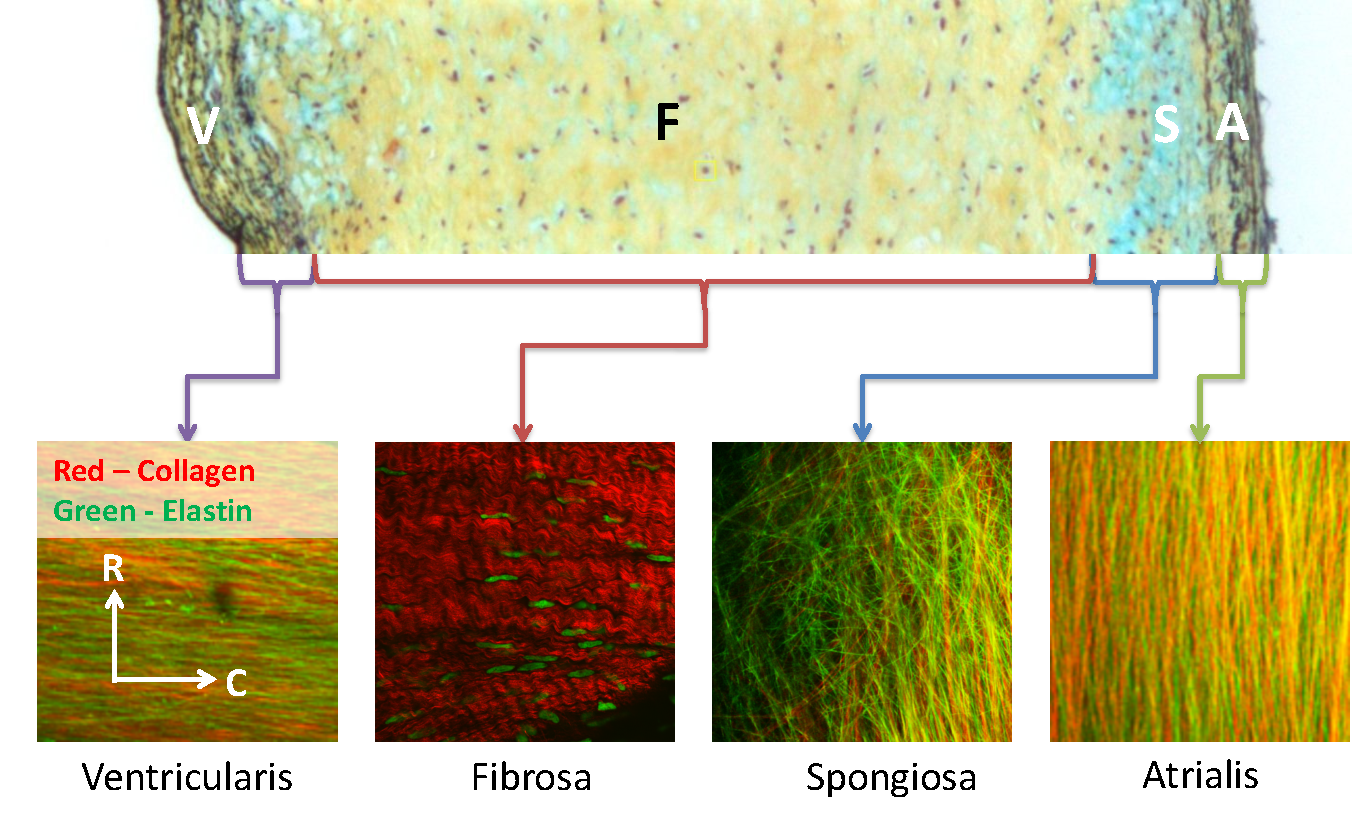
\includegraphics[width=\textwidth]{Images/chapter2/figure2.pdf}
\caption{Microstructural analysis was done using Movat pentachrome stain of the transverse-radial section of the center region of the MV anterior leaflet (Top), and multiphoton microscopy (MPM) of the ventricularis (V), fibrosa (F), spongiosa (S) and atrialis (A) layer of the anterior leaflet (Bottom). The histological section shows the relative thickness of each layer, and the MPM shows the orientation or collagen (red) and elastin (green) fibers in each layer.}
\label{c2:fig:2}
\end{figure}
%%%%%%%%%%%%%%%%%%%%	 end FIGURE 	%%%%%%%%%%%%%%%%%%%%



    
\begin{table}
\centering
\caption{Volume fractions of ECM components in MV (unitless)}\label{c2tab:massfractions}
\begin{tabular}{L{.65in}L{0.65in}L{1.05in}L{0.875in}L{0.875in}L{0.875in}}
\hline
\textbf{Leaflet} & \textbf{ECM} & \textbf{Ventricularis} & \textbf{Fibrosa} & \textbf{Spongiosa} & \textbf{Atrialis}   \\
\hline

\multirow{2}{*}{Anterior}
& Collagen  & $0.078\pm0.018$   & $0.839\pm0.021$   & $0.036\pm0.015$   & $0.047\pm0.007$   \\
& Elastin   & $0.487\pm0.039$   & $0.066\pm0.030$   & $0.067\pm0.000$   & $0.380\pm0.036$   \\
\hline
\multirow{2}{*}{Posterior}
& Collagen  & $0.068\pm0.008$   & $0.778\pm0.052$   & $0.043\pm0.018$   & $0.110\pm0.044$   \\
& Elastin   & $0.104\pm0.021$   & $0.067\pm0.017$   & $0.118\pm0.036$   & $0.711\pm0.035$   \\
\hline
\end{tabular}
\end{table}

\subsection{Experimental mechanical studies} \label{c2:sec:mechanicalstudies}

    In order to develop a comprehensive model to simulate the leaflets in both physiological and surgically altered/pathological conditions, it is necessary to explore the MV properties beyond the physiological range. Moreover, no single deformation mode can provide all the data needed for parameter optimization. Thus, the following deformation modes were utilized.


\subsubsection{Uniaxial loading}

    Under uniaxial loading along the circumferential direction, only the highly circumferentially aligned collagen in the fibrosa and ventricularis layers, which constitute the bulk of the MV, is loaded. This aided the preliminary examination of the collagen fibers mechanics, as the contribution of elastin becomes negligible at high stress. To perform these tests, specimens from four anterior MV leaflets were tested under uniaxial strain until failure. Each specimen was cut into 5 by 20 mm stripes with the long axis oriented along the preferred direction (circumferential) of the leaflet. The specimens were clamped at both ends of the long axis with a separation of 13.5 mm to serve as the gauge length. The transverse direction was unconfined and allowed to contract laterally. One end of the clamps was then displaced at a rate of 0.1 mm/s. The tests were manually aborted after the tissue tears. No preconditioning was done and the tissue was not preloaded. To measure the internal strains more accurately, an optical marker tracking method was used \cite{billiar_biaxial_2000}. All testing was done at room temperature in phosphate buffered saline (PBS).


\subsubsection{Equibiaxial planar strain tests}

    EB planar strain kinematics has several important advantages for examining the effective stress-strain relations in MV leaflet tissues. Firstly, like uniaxial testing, the test can be carried out into the MPa range, exceeding physiological stress levels to ensure all collagen fibers are fully recruited. Secondly, as there are no fiber rotations, one can obtain the fiber ensemble response under the assumption of orientation-invariant fiber recruitment \cite{fata_insights_2014,sacks_incorporation_2003,fan_simulation_2014}. This allows direct estimation of the orientation-invariant fiber recruitment function and effective fiber modulus.
    
    
    To obtain the requisite EB strain data, porcine MV specimens were harvested from a local slaughterhouse and immediately transported for testing. 10 mm by 10 mm sections were taken from the center region of each leaflet and mounted to a custom-built biaxial device \cite{grashow_biaxial_2006,grashow_planar_2006} with the circumferential and radial directions aligned to the device axes. The specimens were immersed in PBS and tested at room temperature. The strain was determined via four fiducial markers glued to the central region of the specimen \cite{billiar_biaxial_2000}. The free-floating state was used as the stress-free reference state, while a preload of 1 g was applied for testing purposes. Starting at 10\% strain, each specimen was tested for ten 30 s cycles with the tenth cycle taken as representative. The maximum strain was then systematically increased until a linear stress-strain region was observed. A total of 7 anterior and 7 posterior porcine MV leaflets were tested.


\subsubsection{Full in-plane responses}

    To obtain the necessary mechanical data for full parameter estimation, a comprehensive set of planar biaxial mechanical data was obtained that encompassed the extra-physiological range. Porcine MV specimens were harvested using a protocol similar to the EB strain testing above. Following mounting, these specimens were first preconditioning for 10 cycles at 90 N/m. The specimens were then unloaded, and the post-preconditioned free-floating state was used as the stress-free references state. Similar to the above, a preload of 1 g was applied for testing purposes. For each loading path, the specimens were loaded to a maximum membrane tension of 90 N/m for ten 30 s cycles with the last cycle taken as representative \cite{grashow_biaxial_2006,grashow_planar_2006}. Circumferential ($x_1$) to radial ($x_2$) ratios of $P_{11}:P_{22}$ = 1:2, 3:4, 1:1, 4:3, and 2:1 were used, with two additional extreme loading protocols that represented extra-physiological ranges of 1:10 and 10:1 to evaluate the MSSCM predictive capabilities.
    
    
\subsubsection{Collagen fiber ensemble analysis using SAXS}

    One way we can assess the intrinsic mechanical properties of collagen fibers, dissociated from the effects of crimping, is using fibril-level measurements from SAXS. We thus utilized extant data from a porcine MV study by Liao et al. \cite{liao_relation_2007} to validate the collagen modulus and recruitment. The experiment was performed on MV anterior leaflets specimens, which were loaded under EB stress. SAXS was used at each load step to measure the fibril strain. Experimental details have been provided in \cite{liao_relation_2007}.
    



\subsection{Parameter estimation}

\subsubsection{General considerations}

    Obtaining the true global cost-function minimum can become exceptionally difficult for highly nonlinear models with a large number of parameters, such as equation \ref{eqn:multilayeredstressform}. This will often include issues such as parameter covariance and the presence of local minima. We thus developed the following detailed sequential procedure for parameter estimation using observations from the structure of the MV leaflet (Section \ref{c2sec:structure}).
    
    
    Firstly, the ventricularis is rich in both elastin and collagen, with a relatively narrow ODF and a preferential orientation in the circumferential direction for both fiber types (Fig. \ref{c2:fig:2}). Secondly, the fibrosa, comprising the bulk of the MV leaflet, contains mainly collagen fibers highly aligned to the circumferential direction with almost no elastin except for trace amounts near the spongiosa. Thirdly, the spongiosa contains relatively small amounts of elastin and collagen, both of which are randomly oriented, and is predominately composed of PGs and GAGs. Fourthly, the atrialis contains the largest population of elastin and some collagen, both of which has a narrow ODF and oriented along the radial direction. Fifthly, since the collagen and elastin fibers in the ventricularis and fibrosa were observed to have very similar ODFs, they cannot be separated reliably from a parameter optimization standpoint. Thus, the small amount of elastin in the fibrosa was considered part of the ventricularis elastin, and the collagen in the ventricularis was considered part of the fibrosa collagen. Also, since the collagen and elastin fibers in the ventricularis and fibrosa were found to be identically aligned and orthogonal to the atrialis, their respective preferred directions were fixed during parameter estimation.
    
    
\subsubsection{Modifications for collagen fiber recruitment bounds}

    As observed in both uniaxial and EB strain data (Fig. \ref{c2:fig:3}), a gradual increase in collagen fiber recruitment and a transition to a linear stress-strain response were clearly visible. In preliminary studies of the collagen fiber recruitment probability function $D(E_s)$, we observed that when the lower-bound $E_{lb}$ was sufficiently distant from the mean $\mu_r$, the overall shape of $D(E_s)$ did not change significantly with further decreases in $E_{lb}$. Thus, to reduce the number of parameters, the lower-bound of the distribution was set to $E_{lb} = 0$.
    
    
%%%%%%%%%%%%%%%%%%%%    begin FIGURE     %%%%%%%%%%%%%%%%%%%%
\begin{figure}
\centering
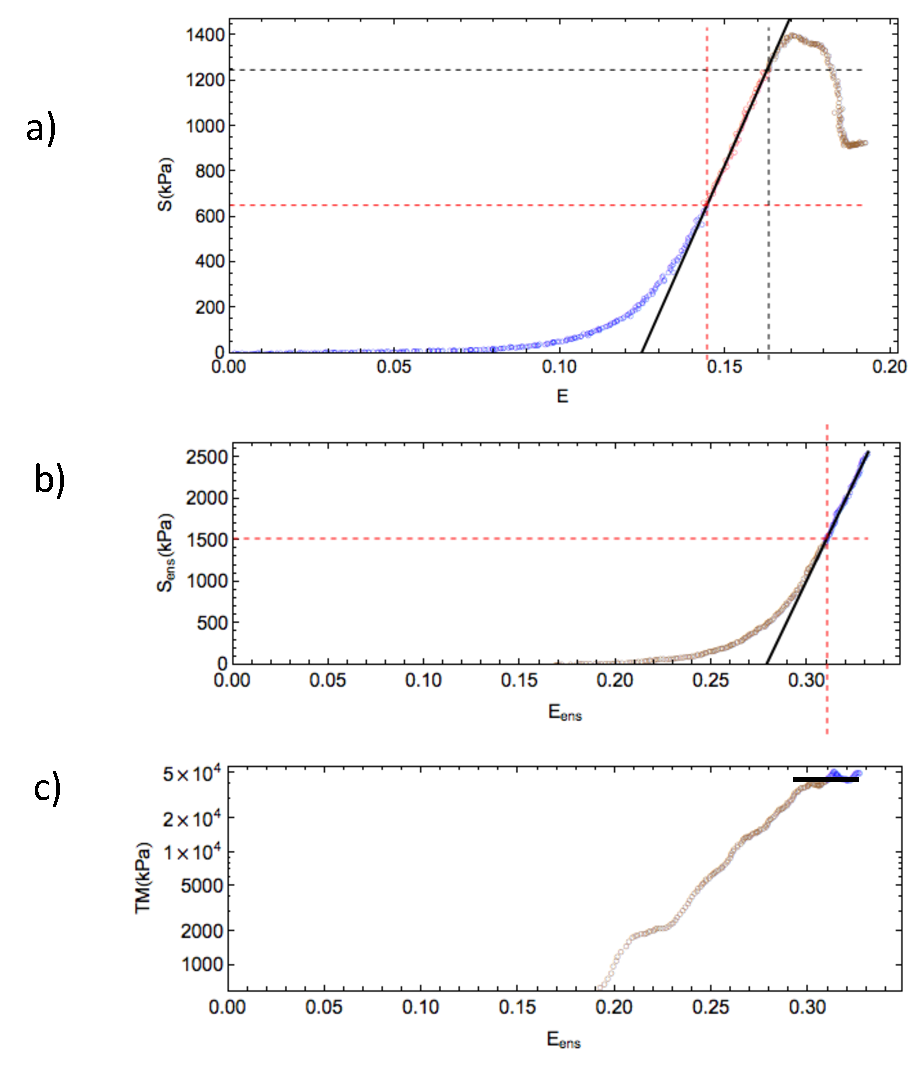
\includegraphics[width=0.95\textwidth]{Images/chapter2/figure3.pdf}
\caption{Example mechanical testing result of (a) uniaxial and (b) and (c) equibiaxial strain test data from an anterior leaflet. The linear post recruitment region is shown by the black line, which indicates full collagen fiber recruitment. The (c) tangent modulus curve in equibiaxial strain test shows a clear flattened section in the post-transition region. Tangent modulus curve for uniaxial extension is not shown due to similarities.}
\label{c2:fig:3}
\end{figure}
%%%%%%%%%%%%%%%%%%%%     end FIGURE     %%%%%%%%%%%%%%%%%%%%




\subsubsection{Elastin fiber model} \label{c2:sec:elastinfibermodel}

    To determine the elastin fiber model (Sections \ref{sec:elastinconsiderations} Elastin fiber network, \ref{sec:collagenconsiderations} Single fiber models), we utilized the low stress region of the mechanical response. Due to the collagen fiber recruitment, we can retroactively determine the Elb of the recruitment distribution as the point when the cumulative distribution is less than 1\% (typically less than 3–8 kPa). Since collagen does not contribute significantly to this region, the response in this region can be considered entirely due to elastin (Fig. \ref{c2:fig:4}a). In pilot studies, we found that $d>1$ in equation \ref{eqn:elastinfiberlaw}. In fact, the exponent for the ventricularis and atrialis layer appeared to be different. Thus, we allowed d to vary during parameter estimation rather than being a set to a constant value.


%%%%%%%%%%%%%%%%%%%%    begin FIGURE     %%%%%%%%%%%%%%%%%%%%
\begin{figure}
\centering
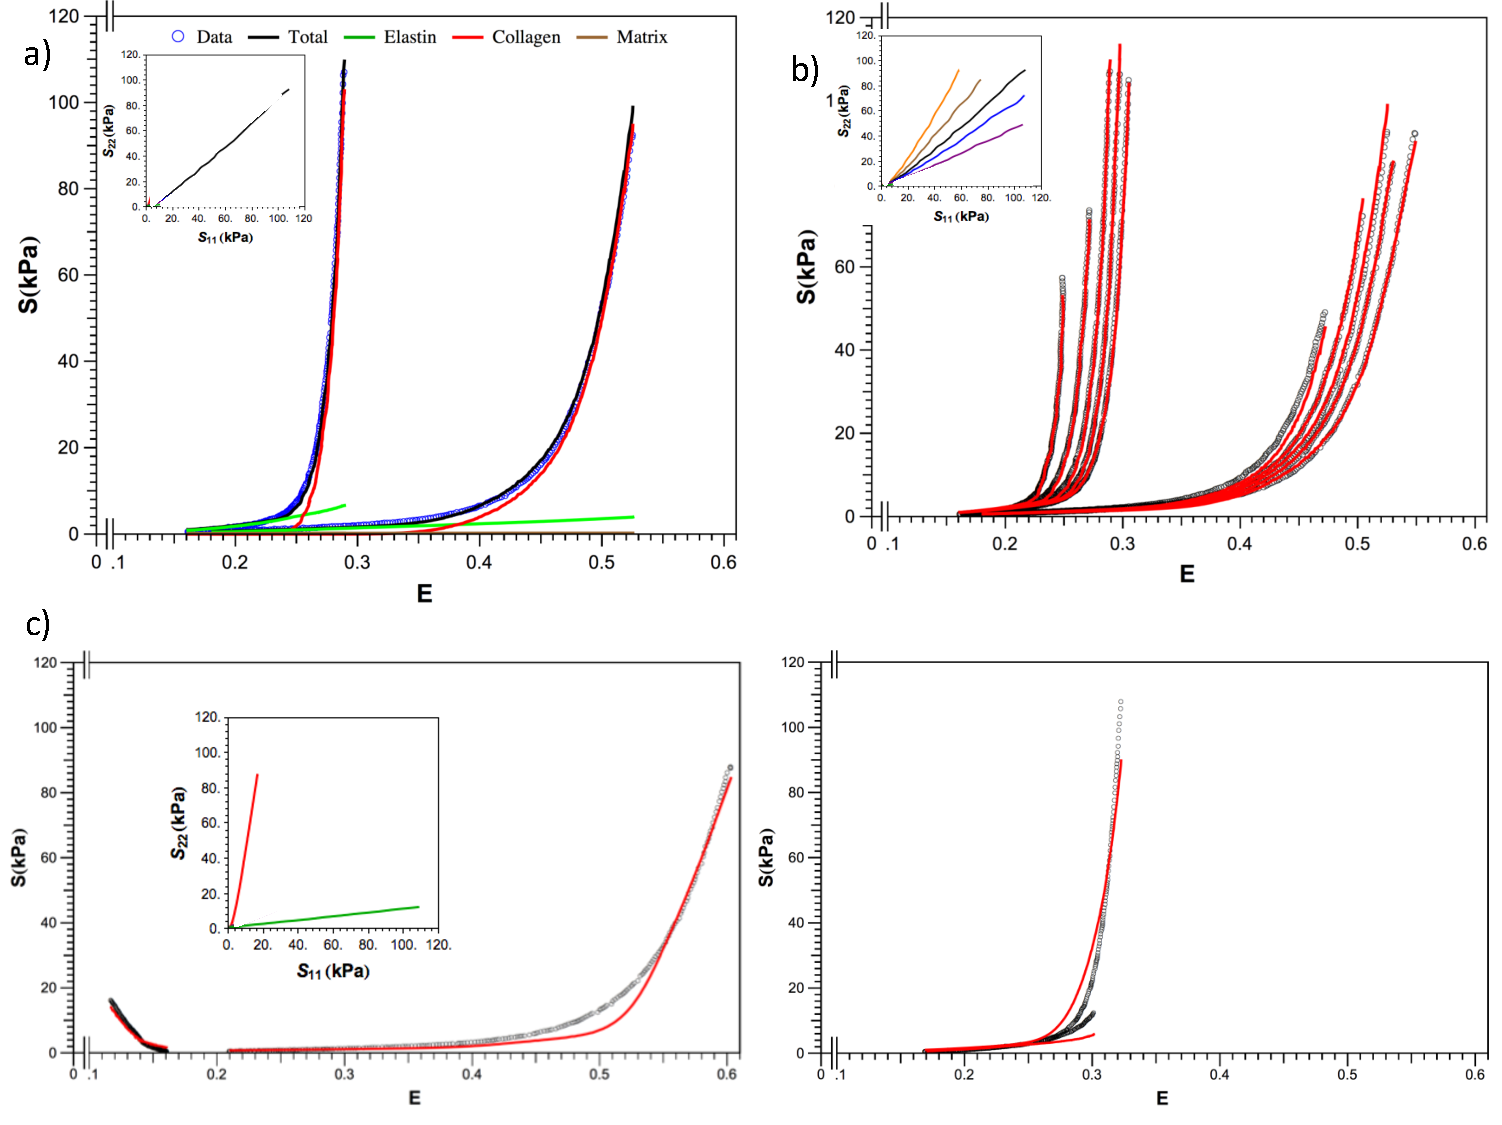
\includegraphics[width=\textwidth]{Images/chapter2/figure4.pdf}
\caption{Example of the best fit from an anterior leaflet. The (a) equibiaxial stress protocol was fit with only the elastin (green) first, followed by fitting the collagen only while keeping the elastin fixed. (b) The final fit of all “physiological” protocols are shown. (c) The two extra-physiological protocols, which were not fit, is shown. This suggests that the model have good predictive capability.}
\label{c2:fig:4}
\end{figure}
%%%%%%%%%%%%%%%%%%%%     end FIGURE     %%%%%%%%%%%%%%%%%%%%




\subsubsection{Parameter estimation part 1 – collagen fiber recruitment} \label{c2:sec:2254}

    From the above analysis, the number of parameters was reduced to 22 (Table \ref{c2tab:modelparameters}). To start with the parameter estimation, we took advantage of the simplified kinematics of the uniaxial and EB test data to isolate the effects of collagen fiber recruitment in a simplified fiber recruitment model. For both datasets, the collagen fiber network in the fibrosa and ventricularis were idealized as a family of uni-directionally aligned fibers, with the elastin fibers neglected as their contributions to the total stress were insignificant in this loading state. Also, note that for the EB tests the fiber ensemble stress can be determined directly by \cite{sacks_biaxial_2000}.
        %-------------------    begin EQUATION     -------------------%
        \begin{equation}\label{c2eqn:ensembleform}
        \begin{aligned}
        S_{ens} = S_{11} + S_{22} \quad \text{for} \quad E_{11} = E_{22}, E_{12} = 0
        \end{aligned}
        \end{equation}
        %-------------------     end EQUATION     -------------------%
    We assumed in this first step that the recruitment distribution is orientation invariant, so that the collagen recruitment function $D(\mathbf{\xi},E_s) = D(\{\mu_r, \sigma_r, E_{lb}, E_{ub}\})$. $E_{ub}$ was determined by the transition point to the linear region (Fig. \ref{c2:fig:3}), leaving only $\mu r$, $\sigma r$ to be fit in this part of the parameter estimation. 
    
    
\subsubsection{Parameter estimation part 2 - full planar biaxial mechanical data set}

    Ideally, the measured ODFs $\Gamma(\theta)$ from the same specimen should be directly inserted into Eqn. \ref{eqn:multilayeredstressform}. However, in practice, we found that the ODFs had to be fitted to adjust for the specimen to specimen variability. Nevertheless, the mean best-fitted ODFs can be compared to the mean measured ODFs to ensure that the estimated parameters are reasonable comparing to the true value. We expedited the process by assuming that the ODFs for each specimen is not significantly different from the true measured mean ODFs. Thus, the mean ODFs can be used as an initial guess and speed up the convergence to the optimal value. The use of a global algorithm will also ensure the optimized parameters do not become trapped at the mean value. Similarly, the estimated recruitment distribution $D(\mathbf{\xi}, x)$ is also obtain from independent specimens. The recruitment distribution parameters $\mathbf{\xi}$ are again used only as initial guesses and parameter validation.
    

    Taking a similar approach to Fata et al. \cite{fata_insights_2014}, we first examined the equibiaxial stress protocol ($P_{11}:P_{22}$ = 1:1), which is the best approximation of the in vivo loading state of the MV. The low stress region as defined in section \ref{c2:sec:elastinfibermodel} was used to fit the elastin (Fig. \ref{c2:fig:4}a). This is easily identified as the nearly linear response before the exponential-like collagen response. Furthermore, due to limitations concerning the elastin model form, where the elastin response can increase exponentially to unrealistically surpass the response of the collagen, the exponent parameter d for the elastin (Table \ref{c2tab:modelparameters}) was constrained to be less than 3.5. Next, the remaining high-stress region was used to fit the collagen fiber response independently. Using this coupled approach, we were able to minimize the search space to the 12 parameters associated with collagen (Table \ref{c2tab:modelparameters}). Once a reliable estimate of the parameters was obtained for this protocol, the inner 3 protocols (3:4, 1:1, 4:3) were fit using the existing parameters as the initial guess. We then progressed to the remaining “physiological” protocols (1:2, 3:4, 1:1, 4:3, 2:1) once again keeping the previous parameters as the initial guess to obtain better-estimated parameters.
    
    
    Preliminary attempts demonstrated that gradient algorithms were unable to converge to the proper solution and tended to become unable to handle local minima. As a result, we employed the genetics-based differential evolution algorithm to perform the optimization, similar to Fata et al. \cite{fata_insights_2014}. To narrow down the search space and guide the optimization, initial guess was derived from the above mechanical studies (Section \ref{c2:sec:mechanicalstudies}). Parameter estimation was performed using a custom program written in Mathematica (Wolfram Research Corp.).
    




\subsection{Model validation} \label{c2:sec:26}

    The mean fitted fiber ODFs $\Gamma(\theta)$ from each layer of the MV anterior leaflet were compared to the measured ODFs obtained from SHG imaging (section \ref{c2sec:structure}). Since the orientation of the fibers is referenced to the laboratory testing or imaging configurations for the mechanical and imaging data respectively, which may be different, the preferred direction of the $\Gamma(\theta)$ was rotated to $\mu_\theta = 0^\circ$ to give the appropriate comparison. Next, in the SAXS study \cite{liao_relation_2007}, the average fibril strain for all fibrils in the leaflet, $\bar{\epsilon}_\mathrm{fibril} = \bar{\lambda}_t - 1$, where  is the mean true stretch of the fibrils, was measured. Since the loading protocol was equibiaxial stress ($P_{11}$:$P_{22}$ = 1:1), the tissue was in an anisotropic strain state, with each fiber ensemble experience different ensemble strain. Additionally, the fiber slack strain reduces the effective stiffness of the fibrils at the tissue-level (Eqn. \ref{eqn:collagenfiberlaw}). Hence we needed to incorporate the $\Gamma_c(\theta)$ as well as collagen fiber recruitment distribution ($D(\mathbf{\xi}, x)$) in the SAXS simulations. The correct fiber modulus ($\eta$) is also necessary to determine the tissue-level stress. Therefore, SAXS gives us an independent method to validate the collagen network model used in this study.
    
    
    To simulate the full SAXS response, as compared to those measured by Liao et al. \cite{liao_relation_2007}, we assume standard affine kinematics (section \ref{sec:generalconsiderations}) \cite{lee_presence_2015}. Thus the fibril stretch is equal to the true stretch of the collagen fibers. Using structural parameters determined from parameter estimation, we simulated a population of fibers based on the fiber ODF and collagen recruitment distributions. The fibers were then deformed based on the EB tension protocol. This corresponds to a mean true fiber stretch given by
        %-------------------    begin EQUATION     -------------------%
        \begin{equation}\label{c2:eqn:fibrilstrain}
        \begin{aligned}
        \bar{\lambda}_t = \int_\theta\Gamma(\theta)\left[\int_1^{\lambda_{ens}(\theta)}D(\mathbf{\xi},x)\frac{\lambda_{ens}(\theta)}{x}\dif x\right]\dif \theta
        \end{aligned}
        \end{equation}
        %-------------------     end EQUATION     -------------------%
    The resulting mean fibril strains $\bar{\epsilon}_\mathrm{fibril} = \bar{\lambda}_t-1$ were plotted against the measured tissue-level stresses and compared to the SAXS $\epsilon_\mathrm{fibril}$ \cite{liao_relation_2007}.


\subsection{Statistical testing}

    Standard independent two-sample t-tests were used to determine the statistical significance of the results.



    
    
    
    